\documentclass{article}
% kodowanie: latin2, utf8 lub cp1250
\usepackage[polish]{babel}
\usepackage[utf8]{inputenc}
\usepackage{polski}
\usepackage[T1]{fontenc}
\frenchspacing
\begin{document}
\emph{Złoty podział} wykorzystuje się często w estetycznych, proporcjonalnych kompozycjach architektonicznych, malarskich, fotograficznych itp. Znany był już w starożytności i przypisywano mu wyjątkowe walory estetyczne. Stosowano go np. w planach budowli na Akropolu. Co najmniej od XX wieku wielu artystów i architektów tworzyło swoje dzieła z zachowaniem złotego stosunku - szczególnie w formie złotego prostokąta, w którym stosunek dłuższego boku do krótszego jest równy złotej proporcji - zgodnie z poglądem, że takie proporcje wyglądają estetycznie. Złoty prostokąt może być rozcięty na kwadrat i mniejszy prostokąt o tych samych proporcjach co rozcinany. Matematycy, począwszy od Euklidesa, badali złoty podział z powodu jego wyjątkowych i interesujących własności. Złoty podział jest także używany w analizie rynków finansowych, w strategiach takich jak \emph{odbicie Fibonacciego}.
\\
\begin{center}Dwie wielkości a i b są w złotym stosunku $\Phi$, jeżeli:\end{center}
\begin{equation}
\frac{a+b}{a} = \frac{a}{b} = \Phi
\label{eq:pierwsze}
\end{equation}
\begin{center} Równanie \begin{math} \Phi^{2} = 1 + \Phi \end{math} również produkuje łańcuchowy pierwiastek kwadratowy, to znaczy:\end{center}
\begin{equation}
\Phi = \sqrt{ 1+\sqrt{1+{\sqrt{1+{\sqrt{\ldots}}}}}}
\label{eq:drugie}
\end{equation}
\\
\begin{center}Określający wielomian kwadratowy i sprzężony związek prowadzą to wartości dziesiętnych, których części ułamkowe wynoszą $\Phi$:\end{center}
\begin{eqnarray}
\Phi^{2} = \Phi + 1 = 2,618\ldots
\\
\frac{1}{\Phi} = \Phi - 1 = 0,618\ldots
\end{eqnarray}
\\
\begin{flushright}
Na rysunku \ref{fig:prostokat} widać jak wyglądają te proporcje w praktyce. Można powiązać z tym równanie \ref{eq:drugie}.
\\
Na rysunku \ref{fig:kepler} widać jak wyglądają te proporcje w praktyce po raz kolejny. A z tym powiązać równanie \ref{eq:pierwsze}.
\end{flushright}
\newpage
\begin{figure}
\centering
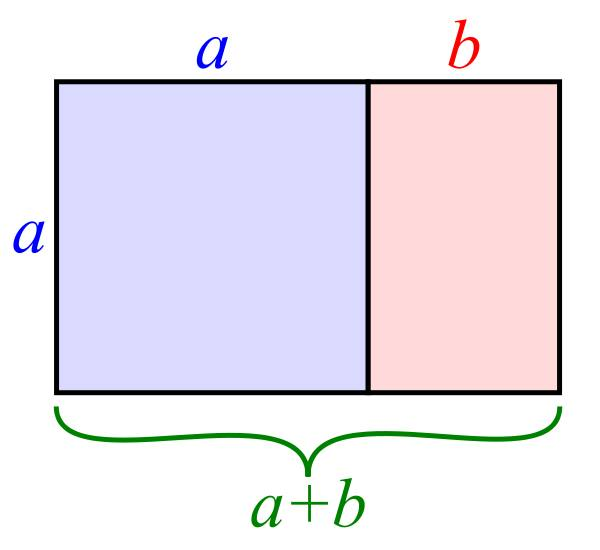
\includegraphics[width=0.5\textwidth, height=0.4\textheight]{grafika/prostokat.png}
\caption{Złoty Prostokąt}
\label{fig:prostokat}
\centering
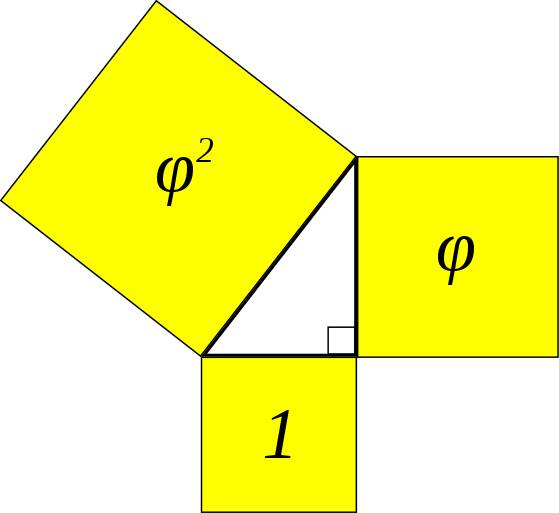
\includegraphics[width=0.5\textwidth, height=0.4\textheight]{grafika/kepler.png}
\caption{Trójkąt Keplera}
\label{fig:kepler}
\end{figure}
\end{document}

